\documentclass{article}
\usepackage[utf8]{inputenc}
\usepackage{graphicx}
\usepackage[margin=1in]{geometry}

\author{Bijan Varjavand, Grace Hao, Kevin Necochea}
\title{Error Analysis - How Stiff is Spaghetti}

\begin{document}

\maketitle
\ \\[2in]
\centering
\section{Abstract}
Mastering basic lab techniques, such as error analysis and dimensionless analysis, is a necessity for Materials Science and Engineering students. By thinking critically about the factors which affect the buckling force of spaghetti with different radii and lengths, we apply skills acquired in the classroom to a practical situation. We learned and used specific techniques in order to quantify unique, mechanical properties of different types of spaghetti. The properties of spaghetti in question are the tensile strength and stiffness. The main technique used was measurement of mass, radii, and length in order to determine the buckling force. However, there is an uncertainty associated with every measurement in this experiment. Error analysis is especially important to our calculations because of our lack of precision and, or accuracy in conducting the measurements. 

\clearpage

\raggedright
\linespread{1.5}
\section{Introduction}
\ \ \ \ \ Spaghetti is a staple in many diets around the world due to its presence in a variety of pasta dishes. This long, cylindrical pasta is a healthy source of carbohydrates, protein and other vitamins.

\ \ \ \ \ Most spaghetti is made from ground grain and water, a mixture which is then dried and packaged for exportation. Distributors must understand the mechanical properties associated with spaghetti in order to limit losses in packaging and processing the material. To accomplish this, they spend time and resources researching how to optimize the mechanical properties of dried spaghetti. Wet and dried spaghetti have very different mechanical properties. Distributors are aware and, thereby, take this into account when generating the final product.

\ \ \ \ \ In schools, teachers choose spaghetti for science projects because it can be used to learn about how materials bend, a subject in which engineers and materials scientists are very interested. Unlike steel beams, spaghetti is highly affordable and it can help students understand concepts such as tension and compression, concepts which can be applied to any material, not just spaghetti. Spaghetti also exhibits visual response to reasonable levels of stress in classrooms.

\ \ \ \ \ In this laboratory experiment, we worked with spaghetti because fairly correct measurements of its mechanical properties can be easily obtained without the need of expensive equipment. We calculated the buckling force associated with three different types of spaghetti at various lengths through compression testing, which can be useful in providing properties such as yield strength, elastic modulus, and ultimate strength.

\ \ \ \ \ Columns under compressive stress can fail in two ways: buckling and crushing. Buckling occurs when a column fails due to bending at a working stress that is less than the ultimate direct stress of the material in question. At this bending point, the force applied can be referred to as the buckling force.
The equation for the buckling force, P, is $$P=E3D464L2$$ where E is the Young’s modulus of the material, L is the length of the sample, and D is its diameter. An important mechanical property, the Young’s modulus is a measure of stiffness of an elastic material, and it can be used to predict elongation or compression.

\section{Error Analysis}

Our buckling load equation is
$$P = \frac{E\pi ^3D^3}{4L^2}$$
$$E = \frac{4PL^2}{\pi ^3D^4}$$

We can confirm the powers by plotting the data on log scales.

\begin{figure}[h]
	\begin{minipage}{0.5\textwidth}
		\centering
		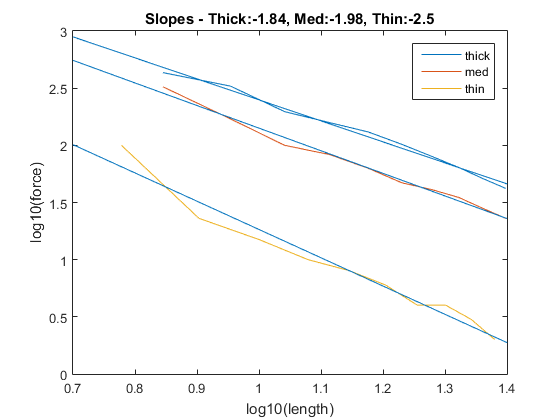
\includegraphics[scale=0.3]{Lab1f1.png}
		\caption{Average for slopes = -2.1}
	\end{minipage}%
	\begin{minipage}{0.5\textwidth}
		\centering
		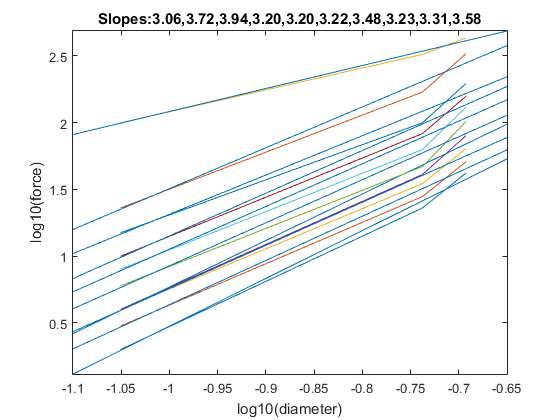
\includegraphics[scale=0.3]{Lab1f3.png}
		\caption{Average for slopes = 3.6}
	\end{minipage}
\end{figure}

Solving for E using our equation, we get 30 values from all our data points. Averaging the E values, we get 2.32 GPa.

The ruler we used had an error of $\pm$ 0.5mm, and the scale had an error of $\pm$ 1g. Converting error from the scale into Newtons, it becomes $\pm$ 0.0098N.

Error propagation given by
$$\frac{\delta E}{E} = \frac{4}{\pi ^3}\sqrt{(\frac{4\delta L}{L})^2 + (\frac{2\delta D}{D})^2 + (\frac{\delta P}{P})^2}$$

$$\frac{\delta E}{E} = \frac{4}{\pi ^3}\sqrt{(\frac{4(0.05cm)}{L})^2 + (\frac{2(0.05cm)}{D})^2 + (\frac{(0.001kg)}{P})^2}$$

I found $\frac{\delta e}{E}$ values for all 30 data points, then averaged all of them to get $\frac{\delta E}{E}$ = 0.0967. Multiplying by the value for E we found, we get $\delta E$ = 224 MPa. This results in $$2.32 \pm 0.22 Gpa$$

\section{Appendix}
\centering
\begin{tabular}{|| c | c | c | c ||}
 \hline
 Thick &\ &\ &\ \\
 \hline
 Length(cm) & Mass(g) & Force(N) & Diameter(cm) \\
 \hline
 \hline
 25 & 42 & 412.02 & 0.203 \\
 23 & 51 & 500.31 &\ \\
 21 & 64 & 627.84 &\ \\
 19 & 80 & 784.80 &\ \\
 17 & 102 & 1000.62 &\ \\
 15 & 131 & 1285.11 &\ \\
 13 & 158 & 1549.98 &\ \\
 11 & 197 & 1932.57 &\ \\
 9 & 329 & 3227.49 &\ \\
 7 & 432 & 4237.92 &\ \\
 \hline
\end{tabular}\\\ \\\ \\\ 

\centering
\begin{tabular}{|| c | c | c | c ||}
 \hline
 Medium &\ &\ &\ \\
 \hline
 Length(cm) & Mass(g) & Force(N) & Diameter(cm) \\
 \hline
 \hline
 25 & 23 & 225.63 & 0.183\\
 23 & 28 & 274.68 &\ \\
 21 & 35 & 343.35 &\ \\
 19 & 41 & 402.21 &\ \\
 17 & 47 & 461.07 &\ \\
 15 & 63 & 618.03 &\ \\
 13 & 83 & 814.23 &\ \\
 11 & 100 & 981.00 &\ \\
 9 & 170 & 1667.70 &\ \\
 7 & 325 & 3188.25 &\ \\
 \hline
\end{tabular}\\\ \\\ \\\ 

\centering
\begin{tabular}{|| c | c | c | c ||}
 \hline
 Thin &\ &\ &\ \\
 \hline
 Length(cm) & Mass(g) & Force(N) & Diameter(cm) \\
 \hline
 \hline
 24 & 2 & 19.62 & 0.089\\
 22 & 3 & 29.43 &\ \\
 20 & 4 & 39.24 &\ \\
 18 & 4 & 39.24 &\ \\
 16 & 6 & 58.86 &\ \\
 14 & 8 & 78.48 &\ \\
 12 & 10 & 98.10 &\ \\
 10 & 15 & 147.15 &\ \\
 8 & 23 & 225.63 &\ \\
 6 & 100 & 981.00 &\ \\
 \hline
\end{tabular}

\end{document}